% !TEX root = ../The-Haptic-Printer.tex
%
\chapter{Features}
\label{sec:concepts}

\cleanchapterquote{A good end product is not just a collection of features, Its how it all works together.}{Tim Cook}{-CEO Apple Inc.}

As mentioned previously the main objective of the application is to consume multiple types of 
inputs from user and render it to the 
Ultrahaptics device. The features are built keeping those multiple inputs in mind. 
A display of multiple inputs can be seen in the image below.
\begin{figure}[htb]
	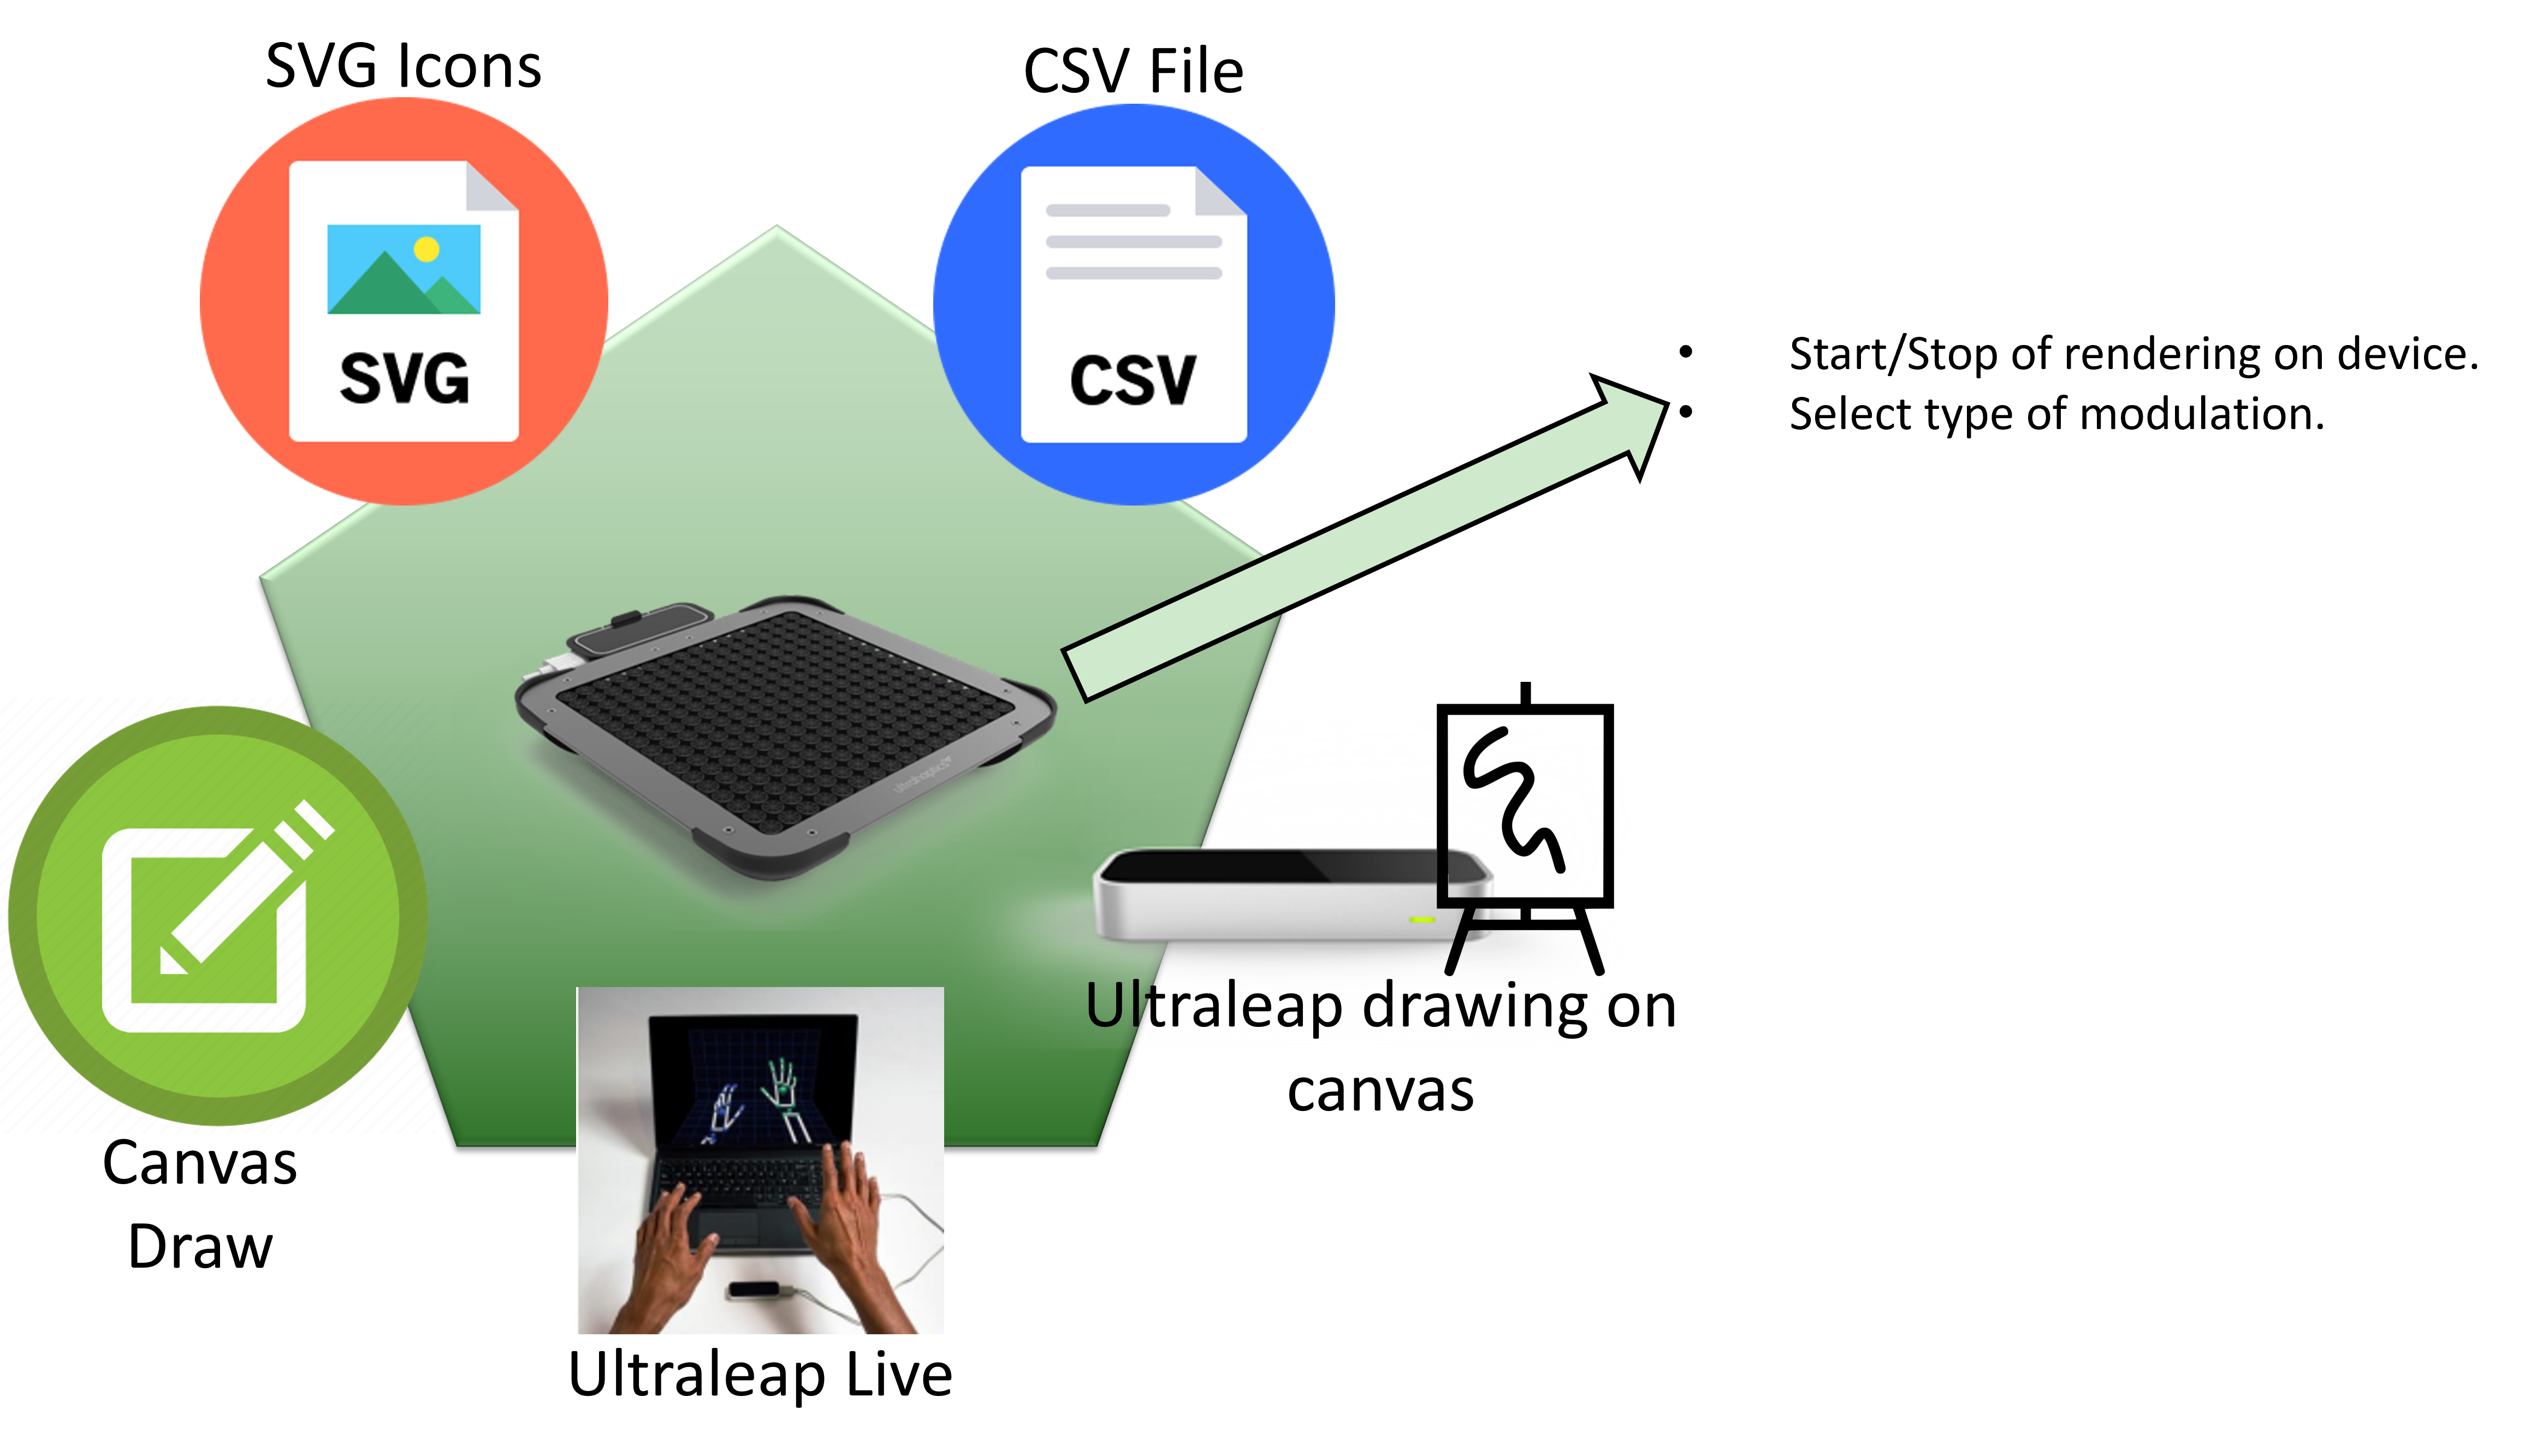
\includegraphics[width=\textwidth]{gfx/Features.png}
	\caption{Figure: Features of the application}
	\label{fig:features}
\end{figure}
The features that are supported in the application are categorized in three part: \\[2mm]
a) Output: Ultrahaptics rendering.\\
b) Inputs: multiple types of inputs supported.\\
c) Controls: how user can control rendering.\\[2mm]
and are explained in brief further on.
% according to the ultrahaptics device
% which should not be over . However, in CSV file the unit is considered to 
% be in meters. For eg. the coordinate (4,5) mm should be 0.004, 0.005 in CSV file.
\section{Output}
Since this application revolves around one major output, it is important to mention 
the output in the beginning. The single output of the application is 
the custom dynamic shape to be rendered/emitted by the ultrahaptics device. 
Since, the device has limited size each input coordinate/s should  be scaled accordingly.

\section{Inputs}
Multiple types of inputs are accepted in the application and tabs are 
created for different inputs, these tabs can be seen in fig 3.2:
\begin{figure}[htb]
	
\includegraphics[width=140mm]{gfx/tabs.jpeg}
	\caption{Figure: Tabs in WebApp}
	\label{fig:features:tabs}
\end{figure}

\subsection*{CSV File}
A CSV file which has the coordinates of points in an x,y plane in column family. 
It can be uploaded in File tab. It assumed that 
the coordinates are mentioned in meters. But since the size of ultrahaptics is 16mm $\times$  16mm
the values in CSV are expected to be in that range. For eg the coordinate (4,5) mm 
should be 0.004, 0.005 in CSV file. An example of the csv input plotted on an xy plane 
can be seen in figure 3.2 only for the visual purpose. \\
\begin{figure}[htb]
	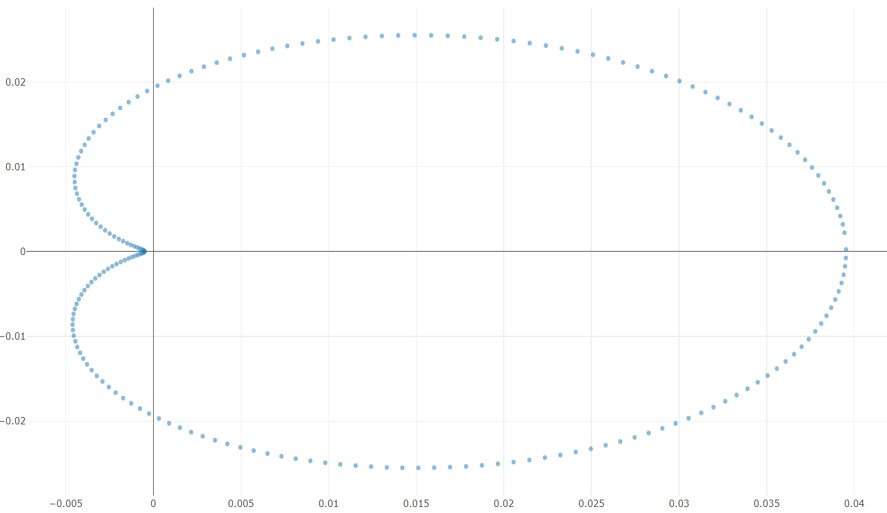
\includegraphics[width=80mm]{gfx/csvinput.jpeg}
	\caption{Figure: example csv Plotted on xy plain}
	\label{fig:features:csvinput}
\end{figure}
In other forms of inputs to the application, the 
coordinates are scaled and centered to size of the Ultrahaptics device by the application. 
However in csv input, it is assumed that the coordinates are scaled and centered.
As soon as the user clicks on the render button the coordinates are 
transferred to the Ultrahaptics device and it starts rendering.


\subsection*{SVG File}
An SVG is also accepted as input format in the same tab as csv. 
As soon as the user uploads the SVG its thumbnail is shown on the 
same page to confirm the visibility. 
SVG coordinates are then communicated to the ultrahaptics device for that shape to
be emitted after user clicks on render button. 


\subsection*{Canvas Draw}
This feature can be accessed under Canvas tab. A HTML 
canvas is provided in which user can draw basic shapes and patterns. 
The coordinates from the canvas is then communicated to the backend and 
rendered on the ultrahaptics device. 

\subsection*{Ultraleap Live}

Ultraleap[ultraleap.com] is an advanced hand tracking  hardware sensory device that accepts hand and 
finger gestures as input, similar to a mouse, but without the need for physical contact.
It is is a tiny USB peripheral device that is meant to be put on a physical desktop 
with its face forward. It's also compatible with virtual reality headsets. 
The gadget observes a roughly hemispheric region to a distance of about 1 meter using 
two monochromatic infrared cameras and three infrared LEDs\cite{s130506380}. The LEDs emit patternless 
infrared light, and the cameras capture almost 200 frames per second of reflected data\cite{leap-controller}. 
This is then transferred to the connected computer via USB connection, where it is processed 
by the company's proprietary hidden code, synthesizing 3D position data by comparing the 
2D frames recorded by the sensors. \\

\begin{figure}[htb]
	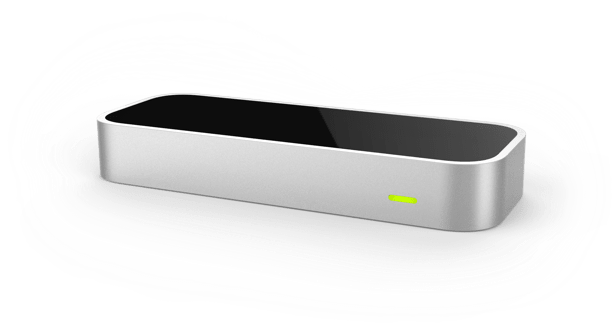
\includegraphics[width=80mm]{gfx/motion-leap.png}
	\caption{Figure: Leap motion controller}
	\label{fig:features:csvinput}
\end{figure}
We consume the data provided by the leap controller and mimic the motion, movement and direction of 
moving index finger on the ultrahaptics board. another requirement of the feature 
is also an ultraleap device connected and 
setup on the system where the webpage is accessed. This feature is accessible in the tab leap 
live. \\

\subsection*{Ultraleap }
Similar to the ultraleap live user can draw shapes on a canvas provided in WebApp
 using the leap motion controller. As soon as the user clicks on render button the 
 shape is rendered on ultrahaptics board. \\[4mm]


\textbf{Note:} To start tracking the index finger by the device on WebApp. First click on the Start Leap 
button provided in our WebApp and then do the click/tap gesture by your index finger above 
Ultraleap motion controller device. 
After that you will get a banner notification that the system is tracking your finger. 
Do the similar gesture to stop the tracking.\\


\section{Controls}
Some basic controls are also provided in the applications where user can secect and 
control other factors, such as:\\
\subsection*{Stop button:} 
On top right of our WebApp a stop button is provided, the rendering on the ultrahaptics 
device can be stopped anytime using this button.\\
\subsection*{Selecting type of rendering:}
On top left of the webapp there is a dropdown select. Here user can switch between
Amplitude Modulation or Time Point streaming for rendering. Once user has selected 
AM, and now wants to observe TPS, rendering has to be stopped by the stop button
before switching.

